
In OpenGL, a 3D point in eye space is projected onto the near plane (projection plane). The following diagrams show how a point $(x_e, y_e, z_e)$ in eye space is projected to $(x_p, y_p, z_p)$ on the near plane.

\begin{figure}[h!]
\centering
\begin{tabular}{cc}
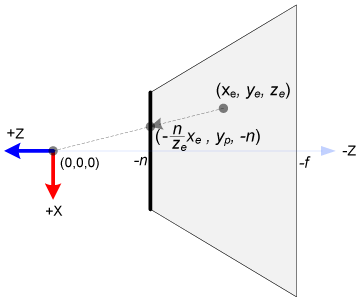
\includegraphics[width=0.45\linewidth,keepaspectratio=true]{figs\gl_projectionmatrix03.png}
&
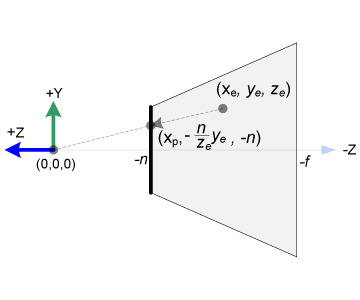
\includegraphics[width=0.45\linewidth,keepaspectratio=true]{figs\gl_projectionmatrix04.png}
\\
(a) Top View of Frustum
&
(b) Side View of Frustum
\end{tabular}
\label{fig.frustum}
\caption{Views of the frustum.}
\end{figure}

From the top view of the frustum, the $x$-coordinate of eye space, $x_e$ is mapped to $x_p$, which is calculated by using the ratio of similar triangles;

\begin{equation}
\begin{aligned}
\begin{split}
\frac{x_p}{x_e}&=\frac{-n}{z_e}\\
x_p&=\frac{-n \cdot x_e}{z_e}\\
   &=\frac{n \cdot x_e}{-z_e}
\end{split}
\end{aligned}
\label{eq.xp}
\end{equation}

From the side view of the frustum, $y_p$ is also calculated in a similar way; 

\begin{equation}
\begin{aligned}
\begin{split}
\frac{y_p}{y_e}&=\frac{-n}{z_e}\\
y_p&=\frac{-n \cdot y_e}{z_e}\\
   &=\frac{n \cdot y_e}{-z_e}
\end{split}
\end{aligned}
\label{eq.yp}
\end{equation}

Note that both $x_p$ and $y_p$ depend on $z_e$; they are inversely proportional to $-z_e$. In other words, they are both divided by $-z_e$. It is a very first clue to construct \verb|GL_PROJECTION| matrix. After the eye coordinates are transformed by multiplying \verb|GL_PROJECTION| matrix, the clip coordinates are still a homogeneous coordinates. It finally becomes the normalized device coordinates (NDC) by divided by the $w$-component of the clip coordinates. (See more details on OpenGL Transformation.) 


\begin{equation}
\begin{aligned}
\begin{split}
\begin{pmatrix} x_{clip}\\y_{clip}\\z_{clip}\\w_{clip} \end{pmatrix} &= 
M_{projection} \cdot \begin{pmatrix} x_{eye}\\y_{eye}\\z_{eye}\\w_{eye} \end{pmatrix}\\
\begin{pmatrix} x_{ndc}\\y_{ndc}\\z_{ndc}\end{pmatrix} &=
\begin{pmatrix} x_{clip}/w_{clip}\\y_{clip}/w_{clip}\\z_{clip}/w_{clip} \end{pmatrix}\\
\end{split}
\end{aligned}
\label{eq.clip}
\end{equation}

Therefore, we can set the $w$-component of the clip coordinates as $-z_e$. And, the 4th of \verb|GL_PROJECTION| matrix becomes $(0, 0, -1, 0)$, using $c$ and $e$ subscripts to refer to the clip and eye coordinates respectively; 

\begin{equation}
\begin{aligned}
\begin{split}
\begin{pmatrix} x_{c}\\y_{c}\\z_{c}\\w_{c} \end{pmatrix} &= 
\begin{pmatrix} 
\cdot & \cdot & \cdot & \cdot \\
\cdot & \cdot & \cdot & \cdot \\
\cdot & \cdot & \cdot & \cdot \\
0 & 0 & -1 & 0 \\
\end{pmatrix} &=
\begin{pmatrix} x_{e}\\y_{e}\\z_{e}\\w_{e} \end{pmatrix}
\end{split}
\end{aligned}
\label{eq.rows}
\end{equation}

Next, we map $x_p$ and $y_p$ to $x_n$ and $y_n$ of NDC with linear relationship; $[l, r] \Rightarrow [-1, 1]$ and $[b, t] \Rightarrow [-1, 1]$.

\begin{figure}[h!]
\begin{center}
\begin{tabular}{cc}
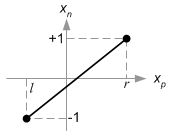
\includegraphics[width=0.45\linewidth,keepaspectratio=true]{figs\gl_projectionmatrix05.png}&
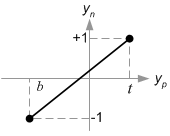
\includegraphics[width=0.45\linewidth,keepaspectratio=true]{figs\gl_projectionmatrix06.png}\\
(a) $x_p$ to $x_n$ relationship & (b) $y_p$ to $y_n$ relationship
\end{tabular}
\label{fig.relationship}
\end{center}
\end{figure}

\begin{equation}
\begin{aligned}
\begin{split}
x_n&=\frac{1-(-1)}{r-l} \cdot x_p+\beta\\
1&=\frac{2r}{r-l}+\beta\\
\beta&=1-\frac{2r}{r-l}=\frac{r-l}{r-l}-\frac{2r}{r-l}\\
     &=1-\frac{r-l-2r}{r-l}=\frac{-r-l}{r-l}=-\frac{r+l}{r-l}\\
     \therefore x_n&= \frac{2x_p}{r-l}-\frac{r+l}{r-l}
\end{split}
\end{aligned}
\label{eq.xn}
\end{equation}

\begin{equation}
\begin{aligned}
\begin{split}
y_n&=\frac{1-(-1)}{r-l} \cdot y_p+\beta\\
1&=\frac{2t}{t-b}+\beta\\
\beta&=1-\frac{2t}{t-b}=\frac{t-b}{t-b}-\frac{2t}{t-b}\\
     &=1-\frac{t-b-2t}{t-b}=\frac{-t-b}{t-b}=-\frac{t+b}{t-b}\\
     \therefore y_n&= \frac{2y_p}{t-b}-\frac{t+b}{t-b}
\end{split}
\end{aligned}
\label{eq.yn}
\end{equation}

Then, we substitute $x_p$ and $y_p$ into the above equations;

\begin{equation}
\begin{aligned}
x_n& = \frac{2x_p}{r-l} - \frac{r+l}{r-l}\\
   &=\frac{2 \frac{n \cdot x_e}{-z_e} }{r-l} - \frac{r+l}{r-l}\\
   &=\frac{2 \cdot n \cdot x_e}{(r-l)(-z_e)} - \frac{r+l}{r-l}\\
   &=\frac{ \frac{2n\cdot x_e}{r-l} }{-z_e}  - \frac{r+l}{r-l}\\
   &=\frac{ \frac{2n}{r-l} \cdot x_e }{-z_e} + \frac{ \frac{r+l}{r-l} \cdot z_e}{-z_e}\\
   &=\underbrace{\left( \frac{2n}{r-l} \cdot x_e + \frac{r+l}{r-l}\cdot z_e\right)}_{x_c} \left.\frac{}{}\left/\frac{}{}\right.\right.-z_e
\end{aligned}
\end{equation}

\begin{equation}
\begin{aligned}
y_n& = \frac{2y_p}{t-b} - \frac{t+b}{t-b}\\
   &=\frac{2 \frac{n \cdot y_e}{-z_e} }{t-b} - \frac{t+b}{t-b}\\
   &=\frac{2 \cdot n \cdot y_e}{(t-b)(-z_e)} - \frac{t+b}{t-b}\\
   &=\frac{ \frac{2n\cdot y_e}{t-b} }{-z_e}  - \frac{t+b}{t-b}\\
   &=\frac{ \frac{2n}{t-b} \cdot y_e }{-z_e} + \frac{ \frac{t+b}{t-b} \cdot z_e}{-z_e}\\
   &=\underbrace{\left( \frac{2n}{t-b} \cdot y_e + \frac{t+b}{t-b}\cdot z_e\right)}_{y_c} \left.\frac{}{}\left/\frac{}{}\right.\right.-z_e
\end{aligned}
\end{equation}

Note that we make both terms of each equation divisible by $-z_e$ for perspective division $(x_c/w_c, y_c/w_c)$. And we set $w_c$ to $-z_e$ earlier, and the terms inside parentheses become $x_c$ and $y_c$ of the clip coordinates.

From these equations, we can find the 1st and 2nd rows of \verb|GL_PROJECTION| matrix. 

\begin{equation}
\begin{aligned}
\begin{split}
\begin{pmatrix} x_{c}\\y_{c}\\z_{c}\\w_{c} \end{pmatrix} &= 
\begin{pmatrix} 
\frac{2n}{r-l} & 0 & \frac{r+l}{r-l} & 0 \\
0 & \frac{2n}{t-b} & \frac{t+b}{t-b} & 0 \\
\cdot & \cdot & \cdot & \cdot \\
0 & 0 & -1 & 0 \\
\end{pmatrix}
\end{split}
\end{aligned}
\end{equation}


Now, we only have the 3rd row of \verb|GL_PROJECTION| matrix to solve. Finding $z_n$ is a little different from others because $z_e$ in eye space is always projected to $-n$ on the near plane. But we need unique $z$ value for the clipping and depth test. Plus, we should be able to unproject (inverse transform) it. Since we know $z$ does not depend on $x$ or $y$ value, we borrow $w$-component to find the relationship between $z_n$ and $z_e$. Therefore, we can specify the 3rd row of \verb|GL_PROJECTION| matrix like this. 

\begin{equation}
\begin{aligned}
\begin{split}
\begin{pmatrix} x_{c}\\y_{c}\\z_{c}\\w_{c} \end{pmatrix} &= 
\begin{pmatrix} 
\frac{2n}{r-l} & 0 & \frac{r+l}{r-l} & 0 \\
0 & \frac{2n}{t-b} & \frac{t+b}{t-b} & 0 \\
\cdot & \cdot & A & B \\
0 & 0 & -1 & 0 \\
\end{pmatrix} \\
z_n &= \frac{z_c}{w_c}= \frac{Az_e+Bw_e}{-z_e}
\end{split}
\end{aligned}
\label{eq.zn}
\end{equation}

In eye space, $w_e$ equals to $1$. Therefore, the equation becomes; 

\begin{equation}
\begin{aligned}
\begin{split}
    z_n &= \frac{Az_e+B}{-z_e}
\end{split}    
\end{aligned}
\label{eq.znreduced}
\end{equation}


To find the coefficients, $A$ and $B$, we use the $(z_e, z_n)$ relation; $(-n, -1)$ and $(-f, 1)$, and put them into the above equation. 

\begin{equation}
\begin{aligned}
    \frac{-An+B}{-n} &= -1 \\
    -An+B &= -n
\end{aligned}
\label{eq.near}
\end{equation}

\begin{equation}
\begin{aligned}
\begin{split}
    \frac{-Af+B}{-f} &= 1\\
    -Af+B &= -f
\end{split}    
\end{aligned}
\label{eq.far}
\end{equation}

To solve the equations for $A$ and $B$, rewrite Equation~\ref{eq.near} for $B$;

\begin{equation}
\begin{aligned}
\begin{split}
    B &= An-n
\end{split}    
\end{aligned}
\label{eq.alfabeta}
\end{equation}


Substitute Equation~\ref{eq.alfabeta} to $B$ in Equation~\ref{eq.far}, then solve for $A$; 

\begin{equation}
\begin{aligned}
\begin{split}
    -Af + (An-n)&=f\\
    -(f-n)A&=f+n\\
    A&=-\frac{f+n}{f-n}
\end{split}    
\end{aligned}
\label{eq.alfa}
\end{equation}

Put $A$ into Equation~\ref{eq.alfabeta} to find B;

\begin{equation}
\begin{aligned}
\begin{split}
    B &= -\frac{f+n}{f-n}n-n\\
      &= -n-\frac{f+n}{f-n}n\\
      &=-\left(1-\frac{f+n}{f-n}\right)n
      =-\left(\frac{f-n+f+n}{f-n}\right)n\\
      &=-\frac{2fn}{f-n}
\end{split}    
\end{aligned}
\label{eq.beta}
\end{equation}

We found $A$ and $B$. Therefore, the relation between $z_e$ and $z_n$ becomes; 

\begin{equation}
\begin{aligned}
\begin{split}
    z_n &= \frac{-\frac{f+n}{f-n}z_e-\frac{2fn}{f-n}}{-z_e}\\
\end{split}    
\end{aligned}
\label{eq.znfinal}
\end{equation}

Finally, we found all entries of \verb|GL_PROJECTION| matrix.